\documentclass{beamer}
\usepackage{amssymb,amsmath}
\usepackage{graphicx}
\usepackage{url}
\usepackage{color}
\usepackage{pagenote}[continuous,page]
\usepackage{cancel}   % Math "cancelto"
\usepackage{relsize}	% For \smaller
\usepackage{url}			% For \url
\usepackage{epstopdf}	% Included EPS files automatically converted to PDF to include with pdflatex

%For MindMaps
\usepackage{tikz}%
\usetikzlibrary{mindmap,trees,arrows}%

%%% Color Definitions %%%%%%%%%%%%%%%%%%%%%%%%%%%%%%%%%%%%%%%%%%%%%%%%%%%%%%%%%
%\definecolor{bordercol}{RGB}{40,40,40}
%\definecolor{headercol1}{RGB}{186,215,230}
%\definecolor{headercol2}{RGB}{80,80,80}
%\definecolor{headerfontcol}{RGB}{0,0,0}
%\definecolor{boxcolor}{RGB}{186,215,230}

%%% Save space in lists. Use this after the opening of the list %%%%%%%%%%%%%%%%
%\newcommand{\compresslist}{
%	\setlength{\itemsep}{1pt}
%	\setlength{\parskip}{0pt}
%	\setlength{\parsep}{0pt}
%}

%\setbeameroption{show notes on top}

% You should run 'pdflatex' TWICE, because of TOC issues.

% Rename this file.  A common temptation for first-time slide makers
% is to name it something like ``my_talk.tex'' or
% ``john_doe_talk.tex'' or even ``discrete_math_seminar_talk.tex''.
% You really won't like any of these titles the second time you give a
% talk.  Try naming your tex file something more descriptive, like
% ``riemann_hypothesis_short_proof_talk.tex''.  Even better (in case
% you recycle 99% of a talk, but still want to change a little, and
% retain copies of each), how about
% ``riemann_hypothesis_short_proof_MIT-Colloquium.2000-01-01.tex''?

\mode<presentation>
{
  \usetheme{CambridgeUS}
  \usecolortheme{dolphin}
  \useoutertheme{default}
  \useinnertheme{default}
  \setbeamercovered{invisible} % or whatever (possibly just delete it)
}
\beamertemplatenavigationsymbolsempty

\usepackage[english]{babel}
%\usepackage[latin1]{inputenc}
\usepackage{subfigure}

\usepackage{times}
\usepackage[T1]{fontenc}
\usepackage{CJKutf8}

%% makes the ppagenote command for figure references at the end.
\makepagenote
\renewcommand{\notenumintext}[1]{}
\newcommand{\ppagenote}[1]{\pagenote[Page \insertframenumber]{#1}}

\title[Experiment Design (01CH740)]{Experiment Design for Computer Sciences (01CH740)}
\author[Claus Aranha]{Claus Aranha\\{\footnotesize caranha@cs.tsukuba.ac.jp}}
\institute[U. Tsukuba]{University of Tsukuba, Department of Computer Sciences}


\subtitle[Experimentalism]{Topic 01 - What is an experiment?}

\begin{document}
\begin{CJK}{UTF8}{ipxm}

\section{Intro}
\begin{frame}
  \maketitle

  \vfill

  \hfill Version 2021.1
\end{frame}

%%%%%%%%%%%%%%%%%%%%%%%%%%%%%%%%%%%%%%%%%%%%%%%%%%%
\begin{frame}{Lecture Outline}
  \begin{itemize}
    \item 1. What is Science?\bigskip

    \item 2. Experimentalism
    \begin{itemize}
      \item What is an experiment?
      \item How do we make a good experiment?
    \end{itemize}\bigskip
    
    \item Description of report 1
  \end{itemize}
\end{frame}

\section{What is Science?}

\begin{frame}
  \begin{center}
    Part I: What is Science -- A discussion based on Examples.
  \end{center}
\end{frame}

\subsection{Definitions}
\begin{frame}{What is Science?}
  At the end of your 2-year course, you will receive a diploma that says:
  \begin{center}
    Master in Computer \structure{Science}
  \end{center}
  What does that word mean?
  \bigskip

  \begin{block}<2>{Some answers from students in past years}
    \begin{itemize}
      \item Science is a method to learn about the world;
      \item Science is a method to reach the truth;
      \item Science is useful when it contributes to society;
      \item Science is how we develop new technologies;
    \end{itemize}
  \end{block}\bigskip

  Give me {\bf your} answer on manaba!
\end{frame}

\begin{frame}{What is Science}{(Not) answering the question}
  \begin{itemize}
    \item All of the answers in the last slide are correct;
    \item "Science" may mean different things to people, depending on their background;
    \item But even the different answers have some common characteristics:
    \begin{itemize}
      \item The discovery of new knowledge;
      \item Understanding the natural world;
      \item Focus on correctness and methodology;
    \end{itemize}
    \item There are also some characteristics that are not often discussed
    \begin{itemize}
      \item Science as a {\bf community}
      \item Science as a {\bf continuous process}
      \item The relationship between {\bf science and society}
    \end{itemize}
  \end{itemize}
\end{frame}

\begin{frame}{What is Science}{I know it when I see it}
  One way that I like to use to understand science, is to look at people who are doing it, and think about what they do.\bigskip

  I think it is important for us to inspire ourselves on the work of other scientists. It is good to have heroes!\bigskip

  So let's talk about \structure{Marie Curie}
\end{frame}

\subsection{Marie Curie}
\begin{frame}{Marie Curie}{Fact Sheet}
  \begin{columns}
    \column{.3\textwidth}
  \includegraphics[width=1\textwidth]{../img/irasutoya_curie}
  \ppagenote{Marie Curie sketch from \url{https://www.irasutoya.com}}\\
    \column{.7\textwidth}

    \begin{itemize}
      \item From Poland, born in 1867, died in 1934.
      \medskip

      \item Physicist and Chemist
      \medskip

      \item Pioneer of radioactivity
      \medskip

      \item First woman to win the Nobel Prize
      \medskip

      \item Only woman to win the Nobel Prize \alert{Twice}
      \medskip

      \item Only person to win the Nobel Prize\\
      \alert{In two different fields}\\
      (Physics and Chemistry)
    \end{itemize}
  \end{columns}
\end{frame}

\begin{frame}{Marie Curie}{Humble Beginnings}
  \begin{columns}
    \column{0.3\textwidth}
    \includegraphics[width=1\textwidth]{../img/marie_curie_sister}\ppagenote{Curie sisters image from Wikipedia (public domain)}\\
    Marie Curie and her sister
    \column{0.7\textwidth}
  \begin{itemize}
    \item Born in Poland
    \medskip

    \item Could not enroll at the local university;\\
      (only accepted men at the time)\medskip

    \item Got educated at the clandestine "Flying University"
    \medskip

    \item Worked as a tutor and home teacher to sustain herself;
  \end{itemize}
\end{columns}
\end{frame}

\begin{frame}{Marie Curie}{Moving to Paris}
  \hfill\includegraphics[width=.3\textwidth]{../img/marie_pierre_curie}\ppagenote{Marie and Pierre Curie image from Wikipedia (Public Domain)}
  \begin{itemize}
    \item Moved to Paris and earned a Physics Degree;

    \item As a researcher, worked in a small shed;
    \item Had difficulty finding research money (funding);
  \end{itemize}
\end{frame}

\begin{frame}{Marie Curie}{Research in Radiology}
  \begin{itemize}
    \item In Marie Curie's time, there was a lot of interest in radioactive materials;
    \begin{itemize}
      \item Why did some materials emit radiation?
      \item What was radiation?
      \item What could we use it for?
    \end{itemize}\bigskip

    \item One of her significant discoveries was that the quantity of radiation depends only on the amount of material;
    \begin{itemize}
      \item This meant that radiation was an \structure{innate property} of radioactive material, not something that was acquired.
    \end{itemize}\bigskip

    \item Marie Curie did not patent the techniques she discovered to study radioactive materials, so that other scientists could also improve their work, and science could progress even faster.
  \end{itemize}
\end{frame}

\begin{frame}{Marie Curie}{Applications of her research}
  \begin{itemize}
    \item Observed that tumour cells died more quickly to radiation than healthy cells;
    \medskip

    \item Developed mobile X-Ray units to be used for surgery during World War I ("little curies")
    \medskip

    \item Developed "Radium Needles" for sterilizing tissue;
  \end{itemize}
  \hfill
\includegraphics[width=0.3\textwidth]{../img/irasutoya_ambulance.png}
  \ppagenote{Ambulance from \url{https://www.irasutoya.com}}
\end{frame}

\begin{frame}{Marie Curie}{Legacy}
  Unfortunately, Marie Curie died early from radiation damage, like many scientists of the time. Her research notebooks are still radioactive, and must be held in special containers!\vfill

  What can you learn from the history of Marie Curie?\bigskip

  What are the scientists that you know? or that inspire you. What can you learn from their history?
\end{frame}

\subsection{Scientific Discoveries}

\begin{frame}

  \begin{center}
    Part II -- The Cycle of Science
  \end{center}

\end{frame}

\begin{frame}{What is Science?}{Scientific Discoveries}
  Science comes in many different forms.\vfill

  Let's discuss two interesting and very different scientific discoveries:
  \begin{itemize}
    \item The cosmic background radiation;
    \item Citrus fruits and scurvy;
  \end{itemize}
\end{frame}

\begin{frame}{Example 1: The Origins of the Universe}
  \begin{itemize}
    \item Physics is a discipline interested in explaining how the universe works. One question of particular interest to physicists is \structure{how the universe began}.\bigskip

    \item One of the most well supported theories for the beginning of the universe is the "inflation theory". According to inflation, the universe started as very dense plasma, and then there was a period of very quick expansion and cooling.\bigskip

    \item Why is the "inflation theory" considered to be well supported? How can we know what happened in the beginning of the universe?
  \end{itemize}
\end{frame}

\begin{frame}{Example 1: The Origins of the Universe}{What evidence supports "inflation"?}

  \begin{columns}

    \column{0.6\textwidth}
    \begin{itemize}
      \item "Inflation Theory" predicted was that for a very short moment,  the universe had expanded enough to be transparent, but was still hot enough to glow.\medskip

      \item The theory allowed a calculation of the duration and intensity of this glow, and that it would be observed from all directions at once.\medskip

      \item Many years later, astronomical radiations actually found evidence for this glow, by accident, which confirmed the theory.\medskip
    \end{itemize}

    \column{0.4\textwidth}
    \includegraphics[width=.9\textwidth]{../img/nasa_cmb}
    \includegraphics[width=.7\textwidth]{../img/nasa_cmb_data}\\
    \ppagenote{CMB images from NASA (public domain)}

  \end{columns}
\end{frame}

\begin{frame}{Example 2: Citrus fruits and scurvy}
  In the 18th century, the British Empire had a very large fleet of ships plundering the entire world.\bigskip

  Maintaining the health of sailors during these long trips was an important issue.\bigskip

  \structure{James Lind}, a scottish doctor, pioneered several ideas to improve naval hygiene. Among those, he conducted a trial to discover how to prevent {\bf scurvy} among sailors.
\end{frame}

% TODO: change CITRUS slide so it does not use a single huge image.
\begin{frame}{Example 2: Citrus fruits prevents scurvy}
  \begin{center}
    \includegraphics[height=.8\textheight]{../img/wikipedia_scurvy}
    \ppagenote{James Lind image from Wikipedia, Public Domain}
  \end{center}
\end{frame}

% \item Understanding Science \url{https://undsci.berkeley.edu/article/intro_01}

\subsection{The Scientific Method}

\begin{frame}{A Framework for Science}{}
  From these examples, we see that the scientific process has some common characteristics.\bigskip

  Many of you might have learned the following description in high school or university:

  \begin{block}{The Scientific Method}
    \begin{enumerate}
      \item Observe a Phenomenom
      \item Propose a Hypothesis
      \item Perform an Experiment
      \item Draw conclusions
    \end{enumerate}
  \end{block}\bigskip

  Is this a good description of "What is Science?"
\end{frame}

\begin{frame}{"The Scientific Method" -- Too simple!}{}
  \begin{columns}
    \column{0.6\textwidth}
      This description of the scientific method has a kernel of truth. But it has some limitations when compared to how science is actually done:
    \column{0.4\textwidth}
      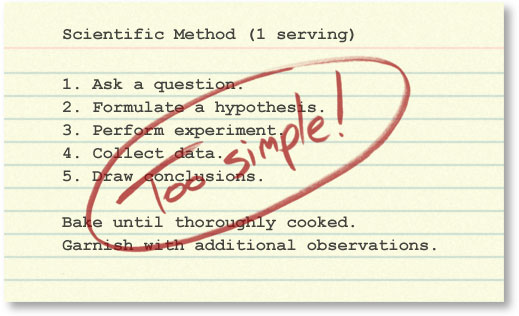
\includegraphics[width=1\textwidth]{../img/scientific_method_simple}
      \ppagenote{"Too simple" image: University of California Museum of Paleontology's Understanding Science}
  \end{columns}
  \vfill

  {\smaller
  \begin{itemize}
    \item It does not explain where questions or hypothesis come from.
    \item What happens when two scientists disagree about the data?
    \item It assumes that the scientific process ends after the data is collected.\\
      \hfill (How does this new knowledge reach society?)\\
      \hfill (How does this new knowledge influence science?)
    \item It assumes that old hypothesis or data never gets reviewed.
    \item etc...
  \end{itemize}
  }
\end{frame}

\begin{frame}{Science as an Interactive Process}{}
  A more complete view of the process of science involves ideas, data, the scientific community, and society, in a continuous feedback circle.
  \begin{center}
    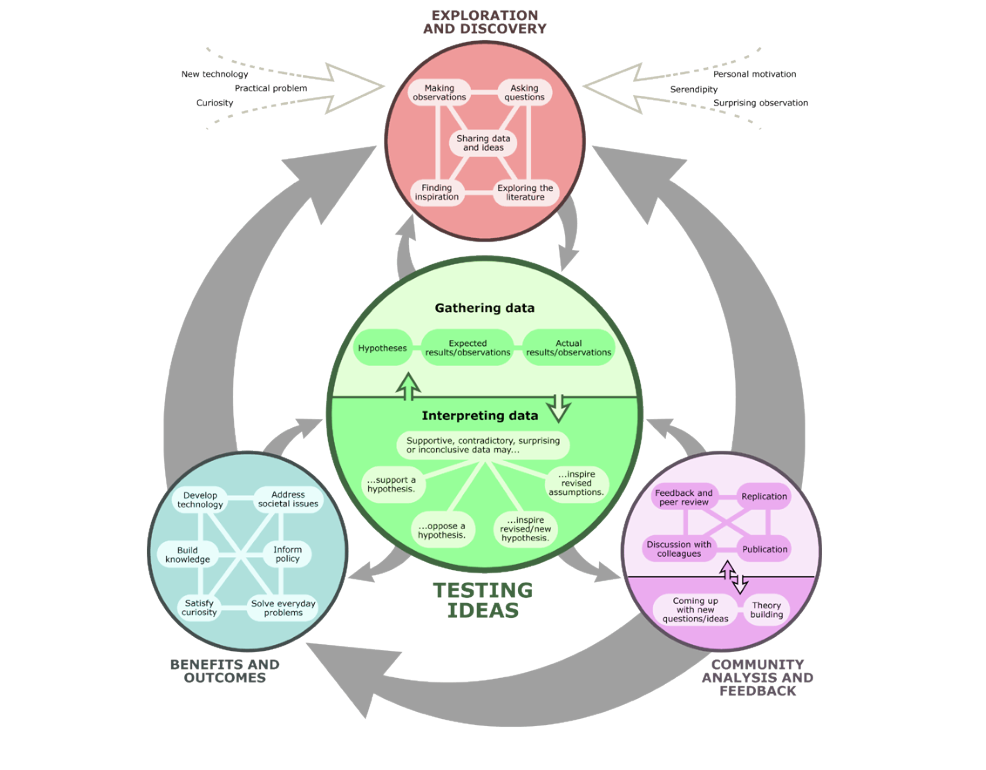
\includegraphics[width=0.5\textwidth]{../img/understandingscience_realprocess1}\ppagenote{"Real Process of Science 1" image: University of California Museum of Paleontology's Understanding Science}
  \end{center}
\end{frame}

\begin{frame}{Science as an Interactive Process}{}
  This understanding helps us see that there are many different paths to scientific discoveries. And these paths still have some common characteristics tying them together.
  \begin{center}
    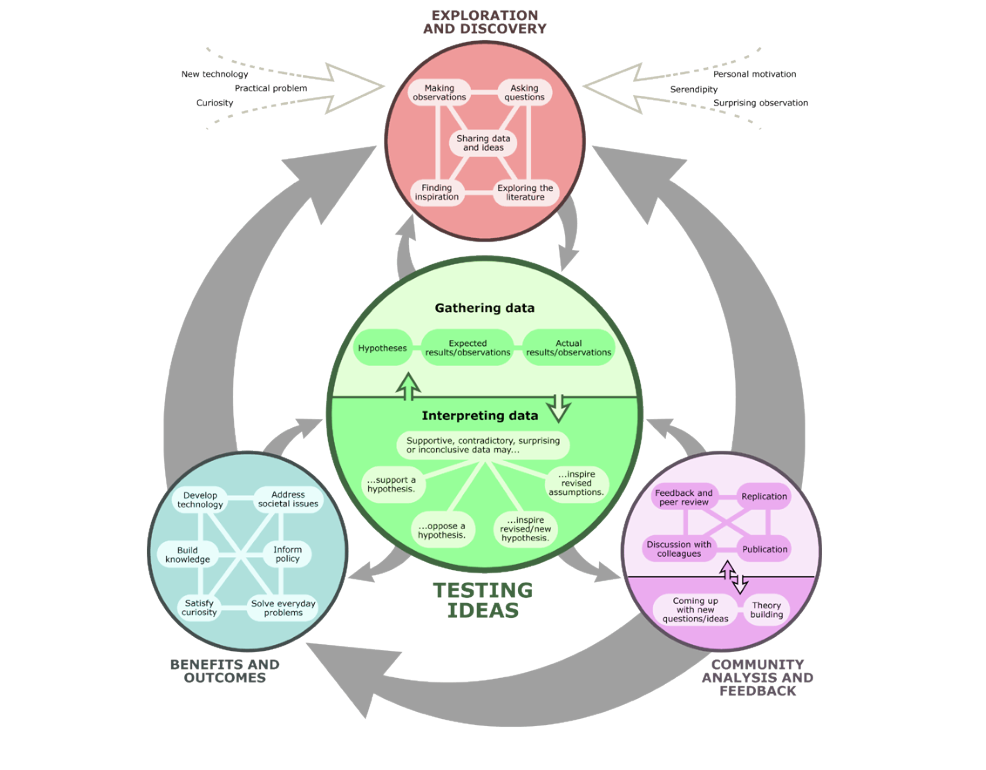
\includegraphics[width=0.5\textwidth]{../img/understandingscience_realprocess1}
    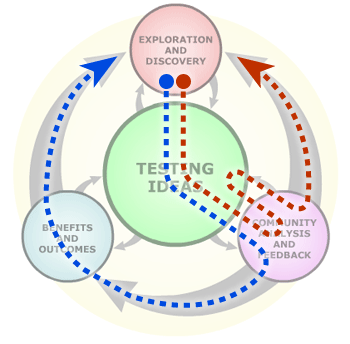
\includegraphics[width=0.4\textwidth]{../img/understandingscience_realprocess2}\ppagenote{"Real Process of Science 2" image: University of California Museum of Paleontology's Understanding Science}
  \end{center}
\end{frame}

\begin{frame}{Science as an Interactive Process -- Breakdown}{Where do ideas come from?}
  \begin{center}
    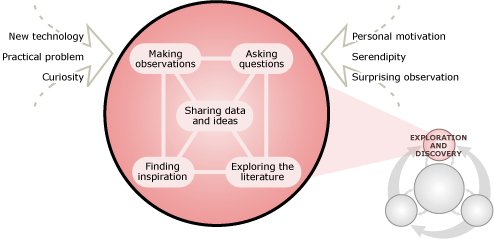
\includegraphics[width=0.8\textwidth]{../img/understandingscience_zoom1}\ppagenote{"Real Process of Science Zoom 1" image: University of California Museum of Paleontology's Understanding Science}
  \end{center}
\end{frame}

\begin{frame}{Science as an Interactive Process -- Breakdown}{Testing and Experimentation}
  \begin{center}
    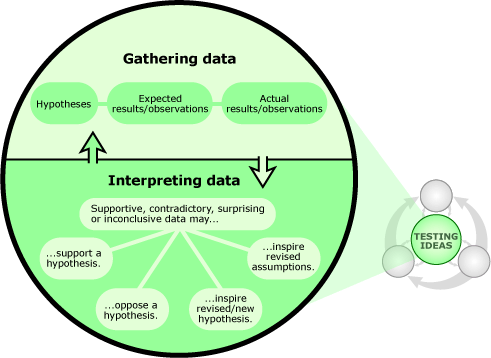
\includegraphics[width=0.6\textwidth]{../img/understandingscience_zoom2}\ppagenote{"Real Process of Science Zoom 2" image: University of California Museum of Paleontology's Understanding Science}
  \end{center}
\end{frame}

\begin{frame}{Science as an Interactive Process -- Breakdown}{The Scientific Community}
  \begin{center}
    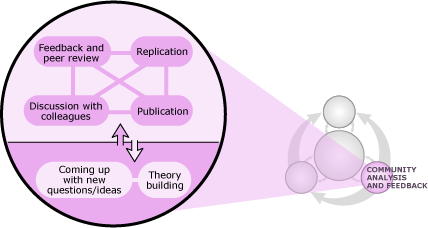
\includegraphics[width=0.8\textwidth]{../img/understandingscience_zoom3}\ppagenote{"Real Process of Science Zoom 3" image: University of California Museum of Paleontology's Understanding Science}
  \end{center}
\end{frame}

\begin{frame}{Science as an Interactive Process -- Breakdown}{Science and Society}
  \begin{center}
    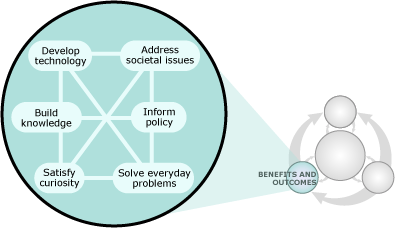
\includegraphics[width=0.7\textwidth]{../img/understandingscience_zoom4}\ppagenote{"Real Process of Science Zoom 4" image: University of California Museum of Paleontology's Understanding Science}
  \end{center}
\end{frame}

\subsection{Wrap-up}
\begin{frame}{Wrap up -- What is Science?}
  \begin{itemize}
    \item Science is a method, a way of thinking, and also a community. A process of search and discovery that is continuously changing our society.
    \item I highly recommend that you read the \structure{"Understanding Science"} webpage, for a much more in-depth discussion. See the manaba links.
    \item {\bf What about Computer Sciences}? Popular discussion of science usually focus on physics, biology, social science, etc. How does Computer Science fit in this framework?
    \vfill

    \item In the next part of the lecture, we are going to focus on the role of experiments in science, which is also the focus for the rest of this class.
  \end{itemize}
\end{frame}


\section{Experimentalism}
\begin{frame}
  \begin{center}
    Part II: Experimentalism
  \end{center}
\end{frame}

\subsection{The Role of Experimentation}
\begin{frame}{The Role of Experimentation}
  \begin{itemize}
    \item Both in the simple definition of the scientific method, and on the more complete one, the experiment takes a central role;
    \bigskip

    \item An experiment is how we test hypothesis, how we learn more about the world, how we examine our ideas;
    \bigskip

    \item But what is an experiment? It is more than just collecting data!
  \end{itemize}
\end{frame}


\section{What is an Experiment?}
% Talk a little bit about Karl Popper
\begin{frame}{What is an experiment?}
  \begin{columns}[t]
    \column{0.8\textwidth}
    \begin{itemize}
      \item Philosophy of Science: How do we obtain knowledge about the world?
      \bigskip

      \item Scientific theories can only be tested by observing their implications;
      \bigskip

      \item Reject theories that cannot be confirmed by experiment;
    \end{itemize}

    \column{0.2\textwidth}
    \includegraphics[width=1\textwidth]{../img/wikipedia_popper}\\
    Karl Popper (1902--1994)
    \ppagenote{Karl Popper picture from Wikipedia}
  \end{columns}
\end{frame}


\begin{frame}{What are the characteristics of a good experiment?}
  \begin{itemize}
    \item Falsifiable Hypothesis;
    \item Useful predictions;
    \item Data Collection;
    \item Reproducibility;
  \end{itemize}
\end{frame}

\begin{frame}{Falsifiability}
  \begin{center}
    \includegraphics[width=0.7\textwidth]{../img/existentialcomics_popper}
    \ppagenote{"Froid and Popper" from \url{http://existentialcomics.com/}}
  \end{center}
\end{frame}

\begin{frame}{Falsifiability}
  \begin{columns}
    \column{0.8\textwidth}
    A scientific hypothesis is {\bf falsifiable} if there is some observation that would render it false.
    \column{0.2\textwidth}
    \includegraphics[width=1\textwidth]{../img/pixabay_whiteswan}
    \ppagenote{White swan image from pixabay}
  \end{columns}
  %% TODO: more specific examples
  \begin{block}{Specific Predictions}
    Falsifiable hypothesis make specific predictions about how the world behaves, not only if the hypothesis is true, but also if the hypothesis were false.
  \end{block}
  \begin{block}{Useful/Strong Predictions}
    It is not very hard to make many trivial predictions about the world. Scientific hypothesis should not only be falsifiable, but also strong and/or useful.
  \end{block}
\end{frame}

\section{Doing Experiments}
\begin{frame}{Types of Experiments}

  There are many different types of experiments, depending on what kind of data you want to obtain. Based on the data collection method, for example, we can classify an experiment in three types:
  \bigskip

  \begin{itemize}
    \item Observational Experiments;
    \item Retrospective Experiments;
    \item Controlled Experiments;
  \end{itemize}
\end{frame}
%% Three types of data collection

\begin{frame}{Types of Experiments}{Observational Experiments}
  In an \structure{Observational Experiment}, you obtain data by observing a phenomena without interacting with it directly.
  \bigskip

  {\bf Example:} you count the number of people who use the train with and without masks every day.
  \bigskip

  \begin{itemize}
    \item Requires care to observe representative situations;
    \item Allows the researcher to choose general conditions for observation;
    \item The situation of interest may be too rare to observe naturally;
  \end{itemize}
\end{frame}

\begin{frame}{Types of Experiments}{Retrospective Experiments}
  In a \structure{Retrospective Experiment}, the researcher obtains data from historical records (newspaper, reports, other scientific papers).\bigskip

  {\bf Example:} you search from the relationship between announcements of celebrity marriages, and total number of registered marriages;\bigskip

  \begin{itemize}
    \item Generally cheaper, and may be the only way to gather data over a very long period of time;
    \item Susceptible to missing records or bias in recording;
  \end{itemize}
\end{frame}

\begin{frame}{Types of Experiments}{Controlled Experiments}
  In a \structure{Controlled Experiment}, the researcher is able to define several variables in the experiment, and perform it in the conditions desired.\bigskip

  {\bf Example:} You develop a new algorithm, and test it on some selected data sets, on a collection of different computational architectures;\bigskip

  \begin{itemize}
    \item Gives a lot of control for the researcher;
    \item If not designed carefully, allows for the introduction of biases into the experiment;
    \item Can be the most expensive kind of experiment (although not always in CS);
  \end{itemize}
\end{frame}


\subsection{Experiment Design}
\begin{frame}{What is Experiment Design?}
  To perform any experiment, we have to make several technical and scientific decisions:
  \begin{itemize}
    \item Which methods we compare in the experiment?
    \item Which data sets are used?
    \item How many times do we interview each participant?
    \item In what order do we perform the experiments?
    \item Which data is reported, and how is the data summarized?
    \item What criteria determines that the hypothesis was accepted or rejected?
    \item What hyper-parameters do we use?
    \item How many times is the experiment repeated? How are these repetitions sumarized?
  \end{itemize}
  {\bf Experiment Design} is how we answer each of these questions.
\end{frame}

%% TODO: Talk a bit about design types? Educated guesses, factorial design, OVAT, etc?

\begin{frame}{Experiment Design}{Example: Controlling for Variation}
  \hfill\includegraphics[width=.2\textwidth]{../img/pixabay_clock}

  Let's say you are comparing two computer programs by measuring their running time (wallclock time).
  \bigskip

  You know that the running time of a program is affected by other programs that are running in the background of the operational system. For example, if a software update happens in the background, it could make a run much slower.
  \bigskip

  To control for this variation, you make sure to run your experiment in a system with a minimum number of running processes, and you also repeat the experiment many times and take the average running time;
  \ppagenote{Clock image from \url{https://pixabay.com}}
\end{frame}

\begin{frame}{Experiment Design}{Example: Controlling for Independence}
  Imagine that you are comparing two website designs with the following experiment: You measure the time for a user to find some information on website A, then you measure the time for website B. \bigskip

  If you make this comparison always in the same order for all users, you discover that the users are a bit faster for website B, because they get used to the testing environment and are more relaxed. \bigskip

  To remove this influence, you make sure that the test order is always random, or you make sure that each user tests only one website.

  \begin{center}
    \includegraphics[width=0.2\textwidth]{../img/irasutoya_website1}\hspace{1cm}
    \includegraphics[width=0.2\textwidth]{../img/irasutoya_website2}
    \ppagenote{Website images from \url{https://www.irasutoya.com}}
  \end{center}
\end{frame}

\begin{frame}{Experiment Design}{Example: Controlling for Fairness}
  You propose a neural network architecture for a new vision problem, and you compare it against traditional architectures.\bigskip

  Because of the special characteristics of the problem, you fine-tune the hyper-parameters of your architecture to achieve the best performance.\bigskip

  To make sure that the comparison is fair, you use the same fine-tune techniques to the traditional architecture that you are comparing against, not using its old hyper-parameters from the literature.

  \hfill\includegraphics[width=0.2\textwidth]{../img/pixabay_neuralnetwork_gordonjohnson}
  \ppagenote{Neural Network image by Gordon Johnson from \url{https://pixabay.com}}
\end{frame}

\begin{frame}{Pre-registered Experiments}
  Pre-registration is the act of fully defining your research protocol {\bf before you begin to collect or analyze data}.
  \bigskip

  By pre-registering your research, you avoid modifying your methods to fit your hypothesis (or modifying your hypothesis to fit your data)
  \bigskip

  Public pre-registration can prevent the loss of negative results. Private pre-registration can help you keep yourself in check.\bigskip

  \begin{columns}
    \column{.7\textwidth}
    Learn more: Center for Open Science \url{https://cos.io/prereg/}
    \column{0.3\textwidth}
    \includegraphics[width=1\textwidth]{../img/prereg-badge}
  \end{columns}
\end{frame}

\subsection{Reproducible Experiments}
\begin{frame}{Reproducible Experiments}
  Reproducibility is an important property of good research:
  \bigskip

  \begin{itemize}
    \item Others can confirm your results;
      \medskip
    \item Others can build on your results;
      \medskip
    \item Others can improve your results;
      \medskip
    \item Society can use your results;
  \end{itemize}
\end{frame}

\begin{frame}{Reproducible Experiments}{How can we make experiments more reproducible?}
  \begin{exampleblock}{Clear Experiment Design}
    Detailed steps taken to perform the experiment; Values of relevant parameters; How the results are processed and evaluated;
  \end{exampleblock}
  \begin{exampleblock}{Open Data and Open Source}
    Data acquisition protocol is clearly defined; Raw data and pre-processing scripts are available; Data is well documented;\bigskip

    For CS, open source of proposed algorithms is essential;
  \end{exampleblock}
  \begin{exampleblock}{Open Documentation}
    Code used for statistical analysis and data visualization;
  \end{exampleblock}
\end{frame}


\section{Outro}

\subsection{Class Summary}
\begin{frame}{Summary of the Lecture}
  \begin{itemize}
    \item Experimentation is a key part of Science;
    \begin{itemize}
      \item Experiments acquires data that can be used to validate or falsify scientific ideas, and to answer scientific questions;
    \end{itemize}
    \bigskip

    \item An experiment has to be performed carefully to guarantee its usefulness;
    \begin{itemize}
      \item {\bf Experimental design} defines the type of experiment, and how data is gathered;
      \item Several factors can affect the {\bf fairness and meaningfulness} of experiments;
      \item {\bf Reproducibility} is essential to guarantee the usefulness of an experiment;
    \end{itemize}
  \end{itemize}

\end{frame}

\begin{frame}{Recommended Reading}
  \begin{itemize}
    \item Understanding Science \url{https://undsci.berkeley.edu/article/intro_01}
    \item Existential Comics \url{http://existentialcomics.com};
    \item Videos: Crash Course Sociology and the Scientific Method, Sociology Research Methods;
  \end{itemize}
\end{frame}

\subsection{Report 01}
\begin{frame}{Report 1}{Design and execute a scientific experiment, and report your results}

  For this report, you must choose a simple experiment to design, perform, and analyze the results. Your report should consist of:\medskip

  \begin{itemize}
    \item {\bf Introduction}: Describe your scientific question, its relevance, and why do you need an experiment for it;
    \item {\bf Experiment Design}: Describe how you will collect data to answer your scientific question; Make sure to mention any parameters or factors that must be controlled;
    \item {\bf Data Collection:} Report on your data collection, if anything happened outside of expected from the experimental design;
    \item {\bf Analysis:} Describe your results in detail, and what answer they provide to your scientific question;
  \end{itemize}
  \begin{alertblock}{}
    \alert{Remember to follow practices of {\bf reproducible science}}
  \end{alertblock}
\end{frame}

\begin{frame}{Report 1}{How to choose an experiment for your report}
  \begin{itemize}
    \item If possible, choose something from your own research;
    \medskip

    \item Experiments from your day to day life are also good;
    \begin{itemize}
      \item Comparing cooking techniques is always fun;
      \item When collecting data, be careful of measuring errors;
    \end{itemize}
    \medskip

    \item When in doubt, comparing algorithms is an easy choice;
    \begin{itemize}
      \item Make sure to choose an appropriate metric to report!
    \end{itemize}
    \medskip

    \item Make sure you choose an experiment that you can perform!
    \bigskip

    \item Next lecture, we will talk about a bit about how to analyze and report experimental data;
  \end{itemize}
\end{frame}



%%%%%%%%%%%%%%%%%%%%%%%%%%%%%%%%%%%%%%%%%%%%%%%%%%%%
\section{Backmatter}
\begin{frame}{About these Slides}
  These slides were made by Claus Aranha, 2022. You are welcome to copy, re-use and modify this material.
  \bigskip

  These slides are a modification of "Design and Analysis of Experiments (2018)" by Felipe Campelo, used with permission.
  \bigskip

  Individual images in some slides might have been made by other
  authors. Please see the following references for those cases.
\end{frame}

\begin{frame}[allowframebreaks]{Image Credits}
  \printnotes
\end{frame}

\end{CJK}
\end{document}
